\subsection{Research design}
In order to answer research questions, I explored more key fields from the initial
database. These fields includes price, date, product type, and shop information.
By applying appropriate statistic on key fields, I produced conclusions based on
numerical results. In addtion, manually discovering the Database market, I captured
a certain of screenshots that support my observation.

In order to replicate my result, please do the following steps:

\begin{enumerate}
    \item Access the original dataset provided by Juha Nurmi at \url{https://
    mega.nz/folder/aJwVyIYJ#}.
    \item Download \emph{database.tar.gz} (7 MB) and follow the instructions
    in \emph{README.md}.
    \item Check \emph{sha256sum}:\\\textbf{5a5f2cb4feb7fee597b0a26b1dc2fb33b1f
    9cae639e995a89663198bcfa76f1a}.
    \item Extract the compressed dataset (tar -xf database.tar.gz).
    \item 33,896 JSON files are generated in the destination folder.
    \item Clone the GitHub repo \url{https://github.com/ancuongnguyen07/Database
    _Market.git} and follow the comprehensive \emph{README.md} document.
\end{enumerate}

%%%%% DATA SAMPLE
\subsection{Samples}
%
The Database Market that sells personal data is accessible through \url{http://d
atabase6e2t4yvdsrbw3qq6votzyfzspaso7sjga2tchx6tov23nsid.onion/} inside the
anonymous Tor network. The initial dataset, provided by teacher Juha Nurmi, can
be downloaded from \url{https://mega.nz/folder/aJwVyIYJ#9SWh-Z3-
TpPfjHZeFxbeew}.
The provided dataset is an archive of 33,896 JSON files, 400 MB of raw size. Each
JSON file is represented as the following fields as shown in \autoref{fig:original_json}:

\begin{itemize}
    \item \emph{url}: URL address of webpage.
    \item \emph{text}: Text of the webpage.
    \item \emph{timestamp}: Data collection date.
\end{itemize}

\begin{figure}
    \centering
    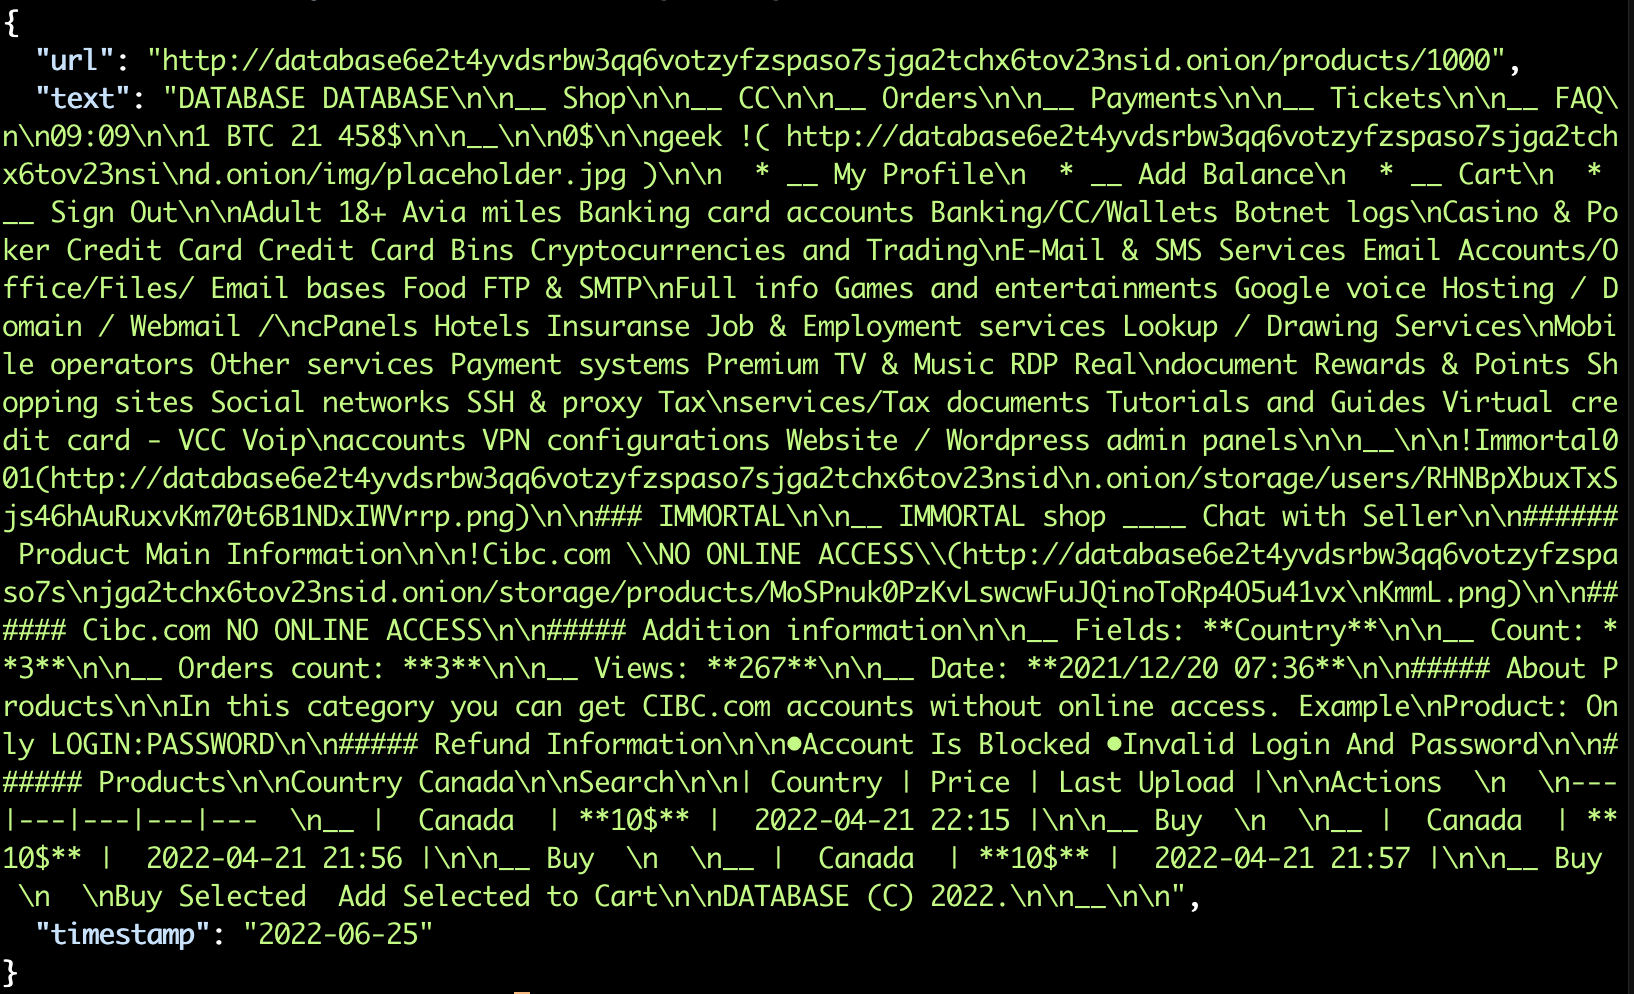
\includegraphics[width=\textwidth,height=\textheight,keepaspectratio]
    {screenshots/orginal_json.png}
    \caption{An example JSON file from the provided dataset by Juha.}\label{fig:original_json}
\end{figure}

In order to achieve more insights of credentials for sale, I produced an additional JSON file
,\emph{ProductPages},that reveals more key features of products sold on a targeted marketplace. Each entry in
the customized JSON file represents a webpage of product containing many sorts of items for sale.
\autoref{fig:custom_json} is an example of an entry, where I assigned the following fields.

\begin{itemize}
    \item \emph{id}: Product ID\@.
    \item \emph{time-stamp}: Data collection date.
    \item \emph{category}: Type of product.
    \item \emph{seller}: Username of seller.
    \item \emph{product}: Name of product.
    \item \emph{prices}: Prices of items.
    \item \emph{dates}: Item uploaded date.
\end{itemize}

\begin{figure}
    \centering
    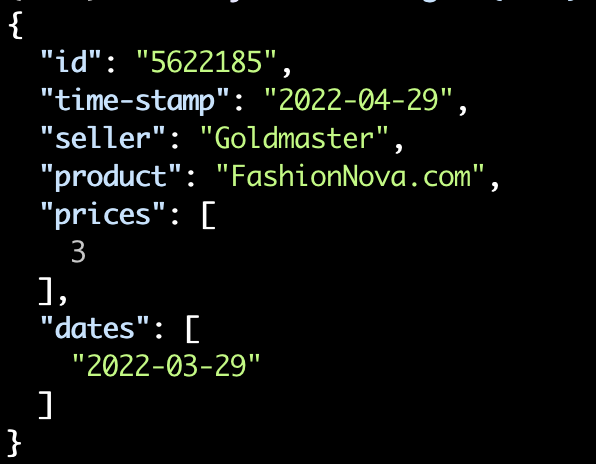
\includegraphics[width=\textwidth,height=\textheight,keepaspectratio]
    {screenshots/customized_json.png}
    \caption{A example JSON entry from my customized dataset}\label{fig:custom_json}
\end{figure}

The datasets are under CC BY 4.0 license: You are free to copy, share, redistribute,
remix, transform, and build upon the material for any purpose, even commercially.
You must give attribution and appropriate credit. Follow the terms: \url{https:/
creativecommons.org/licenses/by/4.0/}.

%%%%% Data collection
\subsection{Data collection}
%
The initial dataset captured web pages of stolen credentials sold in the Database market
from November 2021 to June 2022. Based on that dataset, I extracted a certain of key
fields, including \emph{product, prices, dates} and \emph{seller} for the \emph{text} field.
In addition, I manually took screenshots of pages showing information of products and
stores in Database Market. In order to access a marketplace hosted in Tor network,
it is common that you need an invitation code to register an account on the marketplace.
However, in case of Database Market, I can create an account without an invitation
code.

Filtering interesting fields from the text content in the webpage of product requiring
some marking letters. For example, I noticed that the title of item sold in Database
marketplace is enclosed by ``\#\#\#\#\#\#'', and the store name is covered by ``\#\#\#''. However,
it is more complicated in the cases of \emph{prices} and \emph{dates}. As criminals can
unconstrainedly format the description of their products, I am unable to conduct a common
pattern to capture all prices and dates of uploaded items. Thus, in addition to the quite
effective pattern, returned correct fields in most of pages, I added some criteria for
specific cases. In terms of category, I filtered top common keywords in the title of
products, and grouped items that contain the shared keyword into a category. For example,
any titles containing ``info'', ``ssn'', ``dob'', and ``dl'' belong to the \emph{Personal
data} category.

%%%% Data analysis
\subsection{Data analysis}
%
Applying statistic to the whole dataset, \emph{ProductPages}, I obtained the following
numerical results shown in \autoref{tab:dataset_stat}.

\begin{table}
    \centering
    \begin{tabular}{|c|c|}
        \hline
        Total number of items & 53815\\
        Total number of stores & 30\\
        Maximum price & 2500.00 USD\\
        Minimum price & 0.20 USD\\
        Average price & 15.87 USD\\
        Median price & 5.00 USD\\
        \hline
    \end{tabular}
    \caption{Statistical result of the \emph{ProductPages} dataset.}
    \label{tab:dataset_stat}
\end{table}

The maximum 2500 USD, or other prices greater than 1000 USD, appears with a low
frequency, an outlier. In this case, 2500 USD is a price of a set of 1000 personal data
entries. On the other hand, the average price of personal data is 7.73 USD shown
in \autoref{tab:category_stat}. The price of personal data item depends on the amount
of data pieces included. For example, in the product ID 978, 100 USA \acrshort{ssn}+\acrshort{dob}
is sold at 80 USD, while a buyer has to purchase 250 USD to retrieve 500 USA \acrshort{ssn}+\acrshort{dob}.
In addition, the quality of identity information, also influences
the price. For example, in the product ID 5507764, a set of \acrshort{ssn}+\acrshort{dob}+\acrshort{dl}+\acrshort{mmn}
is sold at 5 USD, while a batch of \acrshort{ssn}+\acrshort{dob}+\acrshort{cs} in ID 5434366 is
assigned at 7 USD\@. The quality of identity information here is interpreted as the level
of financial impact and the simplicity to expose other credential data if this
information is compromised.

There are a certain of product types are traded in Database marketplace. However,
two main categories that most of traded items belong to are \emph{Personal data}
and \emph{Online account}, as shown in \autoref{fig:type_allocation}. \emph{Online
account} category contains compromised online accounts from popular services,
including \textit{Netflix}, \textit{Amazon}, \textit{Venmo}, etc. A full list
of attacked websites is accessible via \url{https://github.com/ancuongnguyen07/
Database_Market/blob/main/analysis_result/leaked_websites.txt}.

There are in total 30 stores, or sellers, in the database. \emph{Goldmaster}, the
most active seller, has sold the largest amount of products during 11/2021--06/2022,
11882 items. However, \emph{bussman shop}, a store that has the greatest average price (430 USD),
only sold 9 items. Furthermore, \emph{bussman shop}, provides service of customizing
ID documents for \acrshort{eu}/\acrshort{us}; thus, the prices of it's products are significant
higher than those of other shops, ranging from 80 USD to 1200 USD\@. A table of full
numerical results from analyzing stores is accessible in \url{https://github.com/anc
uongnguyen07/Database_Market/blob/main/analysis_result/seller_stat.csv}.

\begin{figure}
    \centering
    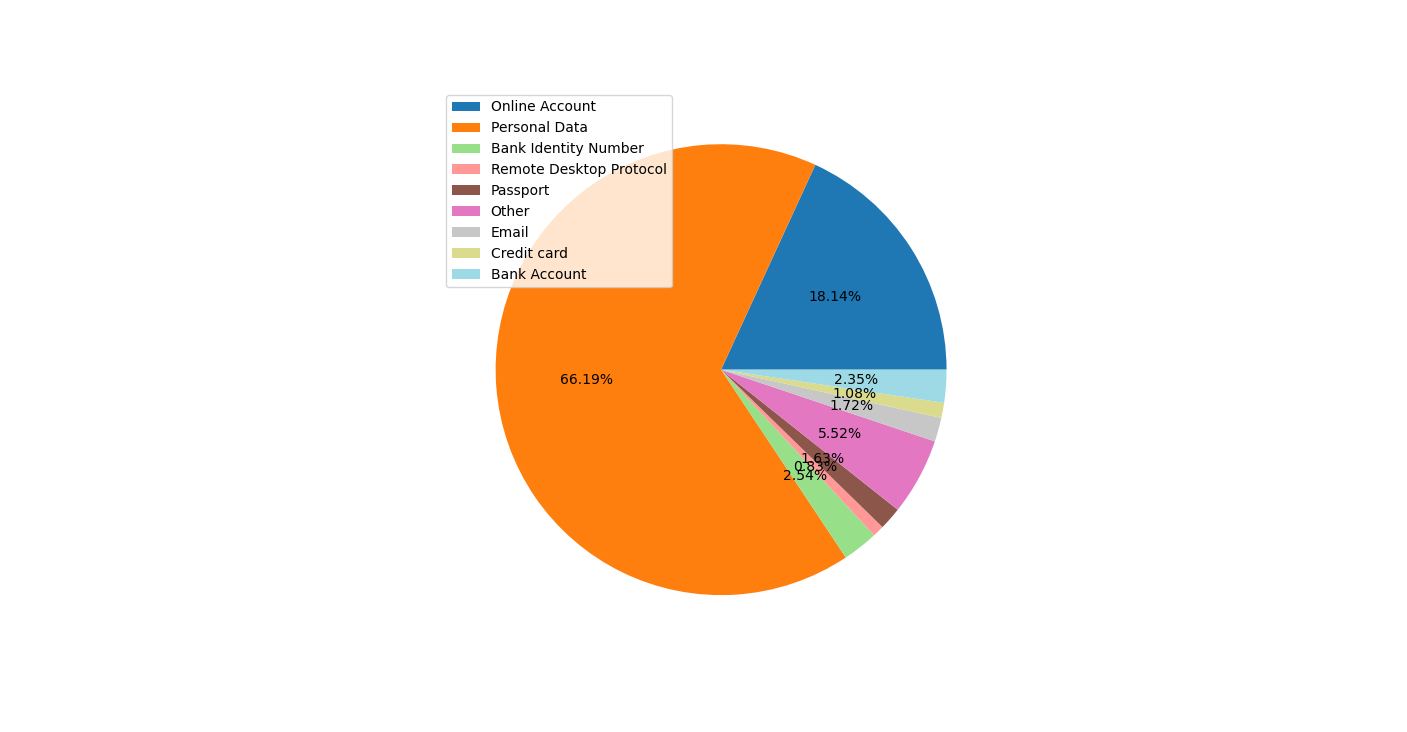
\includegraphics[height=\textheight,width=\textwidth,keepaspectratio]
    {plots/category_allocation.png}
    \caption{Product types allocation.}\label{fig:type_allocation}
\end{figure}

\begin{figure}
    \centering
    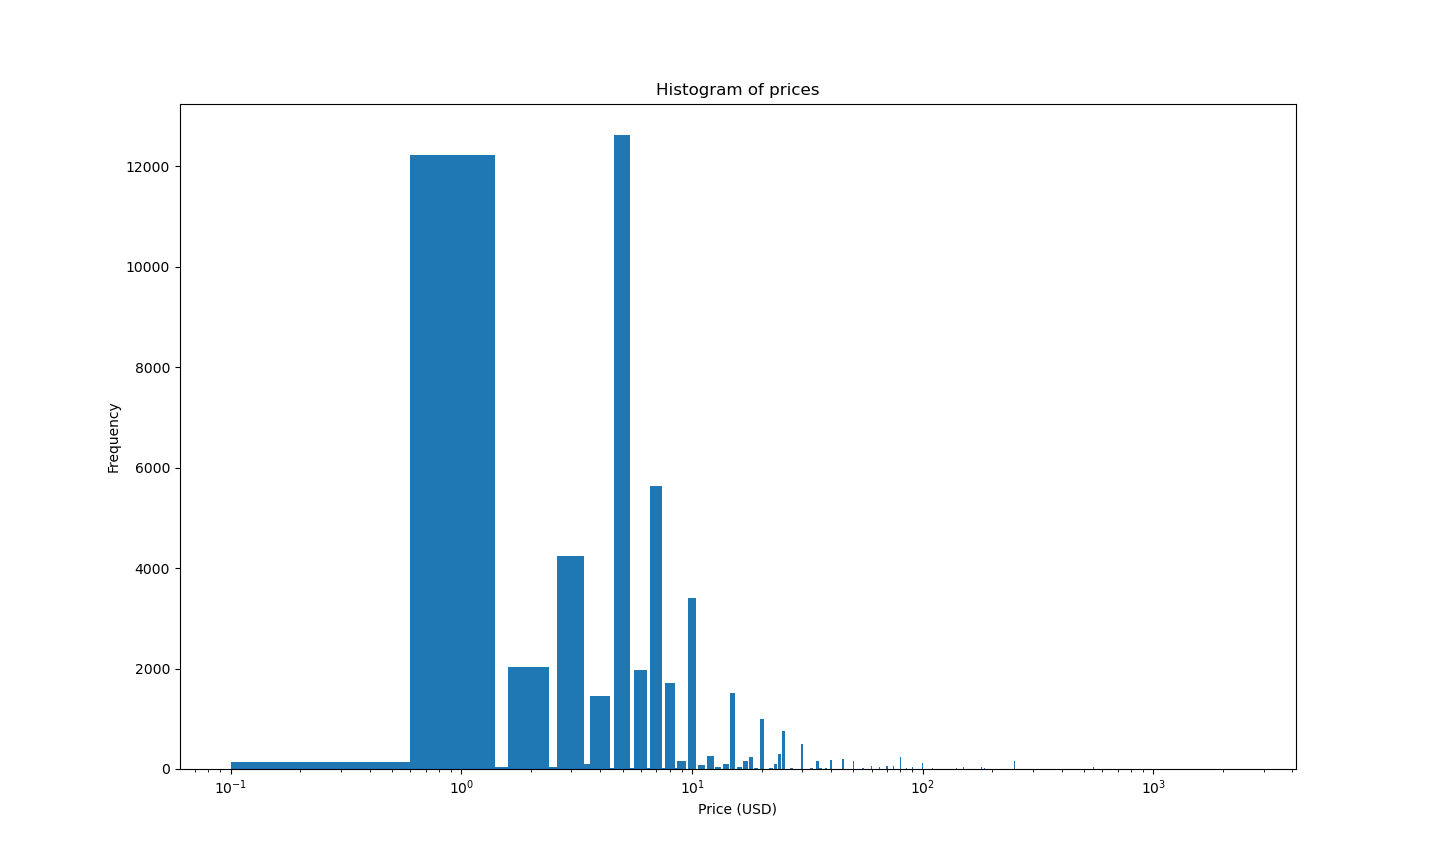
\includegraphics[height=\textheight,width=\textwidth,keepaspectratio]
    {plots/price_histogram.png}
    \caption{Price distribution.}\label{fig:price_range}
\end{figure}

\begin{figure}
    \centering
    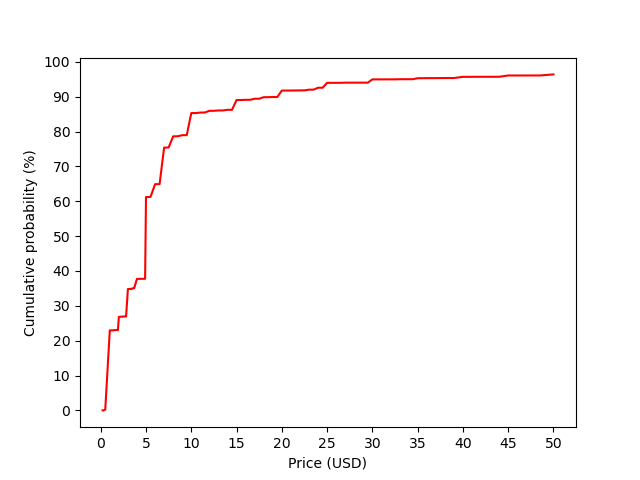
\includegraphics[height=\textheight,width=\textwidth,keepaspectratio]
    {plots/cumprob_price.png}
    \caption{Cumulative probability of price range 0--50 USD.}\label{fig:cum_prob}
\end{figure}

%%%%% Limitation
\subsection{Limitations}
% time range is so far from this moment
The initial database recorded product information in 8 months, from November 2021
to June 2022, covering 33896 product pages. First, the time of writting this study,
November 2022, is 5-month after the last captured product in the database; therefore,
observations and propositions instroduced in this study do not provide the most
updated status of the Database marketplace. In comparison to product entries in
the original database, the marketplace now provides more items; and many products
recorded in the database is now either withdrawed or sold out, i.e product ID
5609797 (\autoref{fig:not_found_prod}).

\begin{figure}
    \centering
    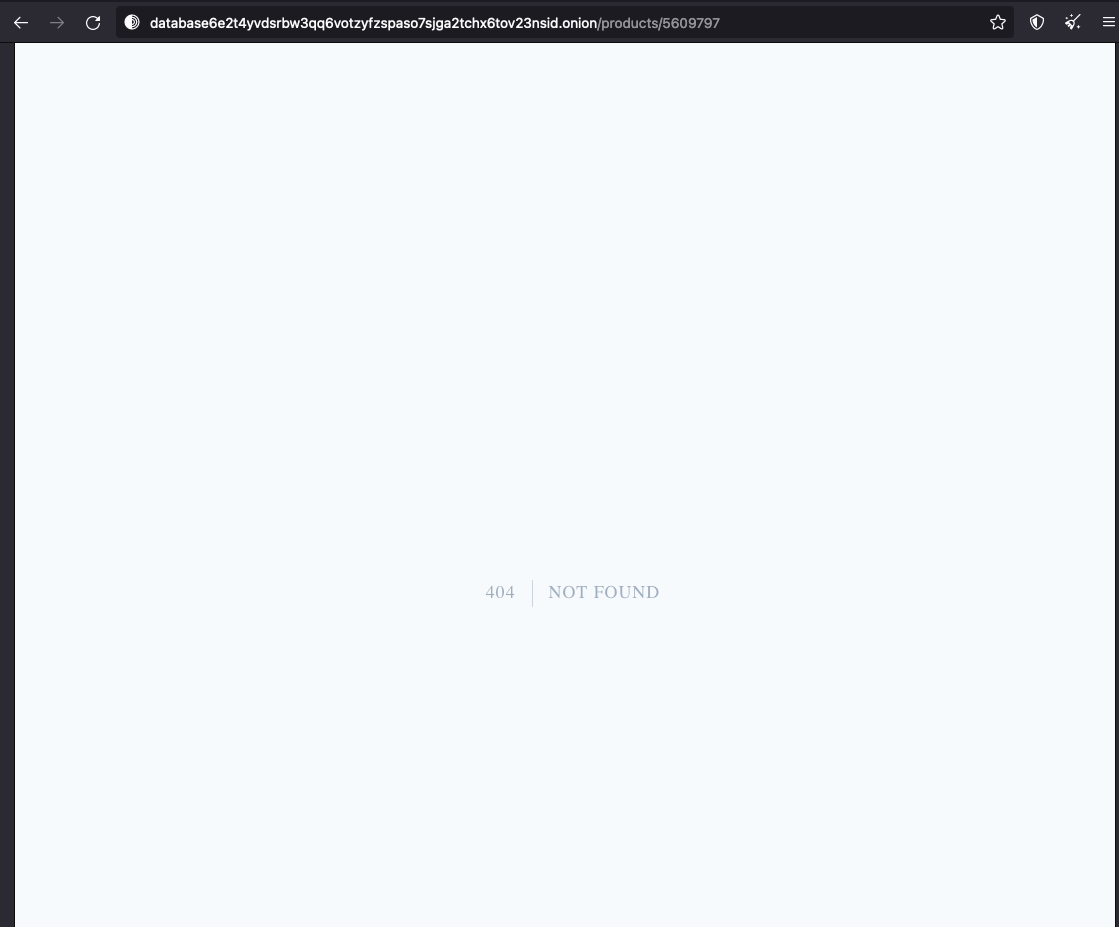
\includegraphics[height=\textheight,width=\textwidth,keepaspectratio]
    {screenshots/not_found_prod.png}
    \caption{Withdrawed/sold-out product ID 5609797.}\label{fig:not_found_prod}
\end{figure}

% seller can freely format product description
In Database marketplace, shops can unconstrainedly format their product description;
thus, I cannot filter exactly interesting fields in all cases, resulting minor noise
in the examination.
% group category manually, by personal preference
Moreover, product category is not provided in the inital database, not even in the
product page. In order to attain product type data, I grouped products that have
the common keywords in a category as presented in \autoref{tab:category_stat}.
This text-based clustering method is not reliable in all cases.

% no feedback information of seller
I examined that there is a shortage of feedback information about stores, or sellers, in
the Database market. As shown in \autoref{fig:seller_asap_market}, in the ASAP marketplace,
feedbacks from customers are classified as negative and positive, that is helpful
to detect an unreliable shop. On the other hand, as presented in \autoref{fig:seller_Database},
Database market does not display feedbacks a specific store, but buyers can send
comments via the internal ticket which is not shown in the store dashboad.

\begin{figure}
    \centering
    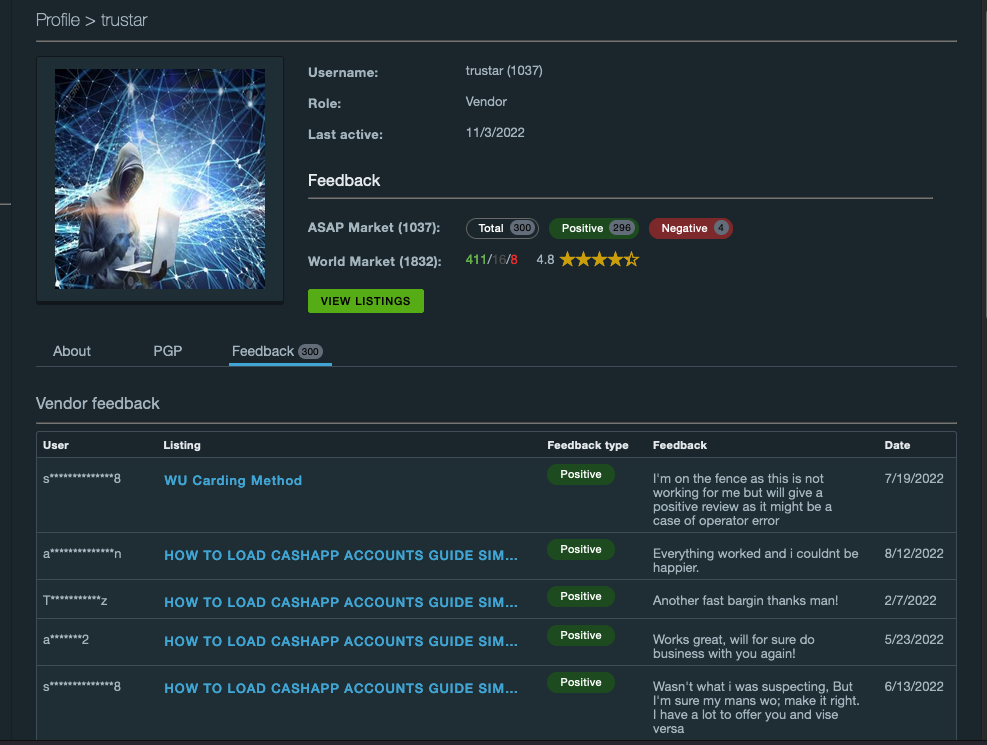
\includegraphics[height=\textheight,width=\textwidth,keepaspectratio]
    {screenshots/seller_feedback_asap_marketplace.png}
    \caption{A shop page in ASAP marketplace.}\label{fig:seller_asap_market}
\end{figure}

\begin{figure}
    \centering
    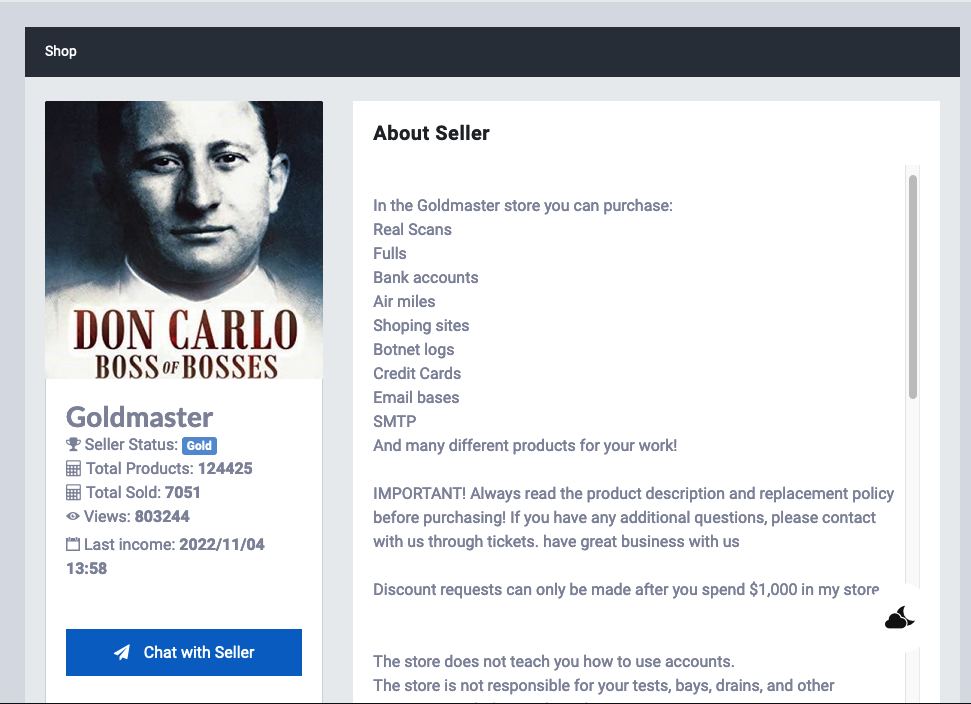
\includegraphics[height=\textheight,width=\textwidth,keepaspectratio]
    {screenshots/seller_page.png}
    \caption{A shop page in Database marketplace.}\label{fig:seller_Database}
\end{figure}